%!TEX root = ../quantum.tex
\subsubsection{Вопрос 2}
Напишите разложение единичного оператора по собственным векторам к.л. оператора.

Пусть есть некий оператор $\widehat{A}$.
$$\widehat{A}\ket{\psi_n} = a_n \ket{\psi_n},$$
где $\ket{\psi_n}$ - собственный вектор оператора.

В абстрактных обозначениях: $\ket{\psi_n} = \ket{n}$. Тогда
$$\widehat{1}=\sum_n C_n \ket{n}$$
Умножим скалярно на $\bra{\psi_m} = \bra{m}$
$$\bra{m} \widehat{1}=\sum_n \bra{m} C_n \ket{n}$$
Но если $m\neq n$, то $\ket{\psi_n}$ и $\ket{\psi_m}$ ортогональны. Следовательно, сумма отлична от нуля только при $m=n$ 
$$\bra{n} \widehat{1}=C_n, \bra{m}\widehat{1}=\bra{n}$$
$$\widehat{1}=\sum_n \ket{n} \bra{n}$$

\subsubsection{Вопрос 3}
Найдите $\Psi(p)$ по данным $\Psi(x)$. Найдите связь ширины в $x$ и $p$ представлениях. $\Psi(x)=\frac{1}{x^2+a^2}$.
$$\Psi(p)=\frac{1}{\sqrt{2\pi \hbar}} \int_{-\infty}^{+\infty} \Psi(x) e^{\frac{-ipx}{\hbar}}dx$$

1) $Im z>0, \lambda >0$. Используя лемму Жордана:
$$\int_{-\infty}^{+\infty} \frac{1}{x^2+a^2} e^{\frac{-ipx}{\hbar}}dx=2\pi i \sum_{k=1}^n res [R(z)\exp{i \lambda z}],$$
где $R(z)=\frac{1}{z^2+a^2}, \lambda=-\frac{p}{\hbar}$ 

Найдем особые точки 
$$R(z)= \frac{1}{z^2+a^2} = \frac{1}{(z+ia)(z-ia)}$$
$$z_0=\pm ia$$
Особе точки - полюса первого порядка. Внутри контура $L_1$ одна особая точка $z_0=ia$. Для полюса первого порядка

% \begin{wrapfigure}{l}{0.3\linewidth}
% 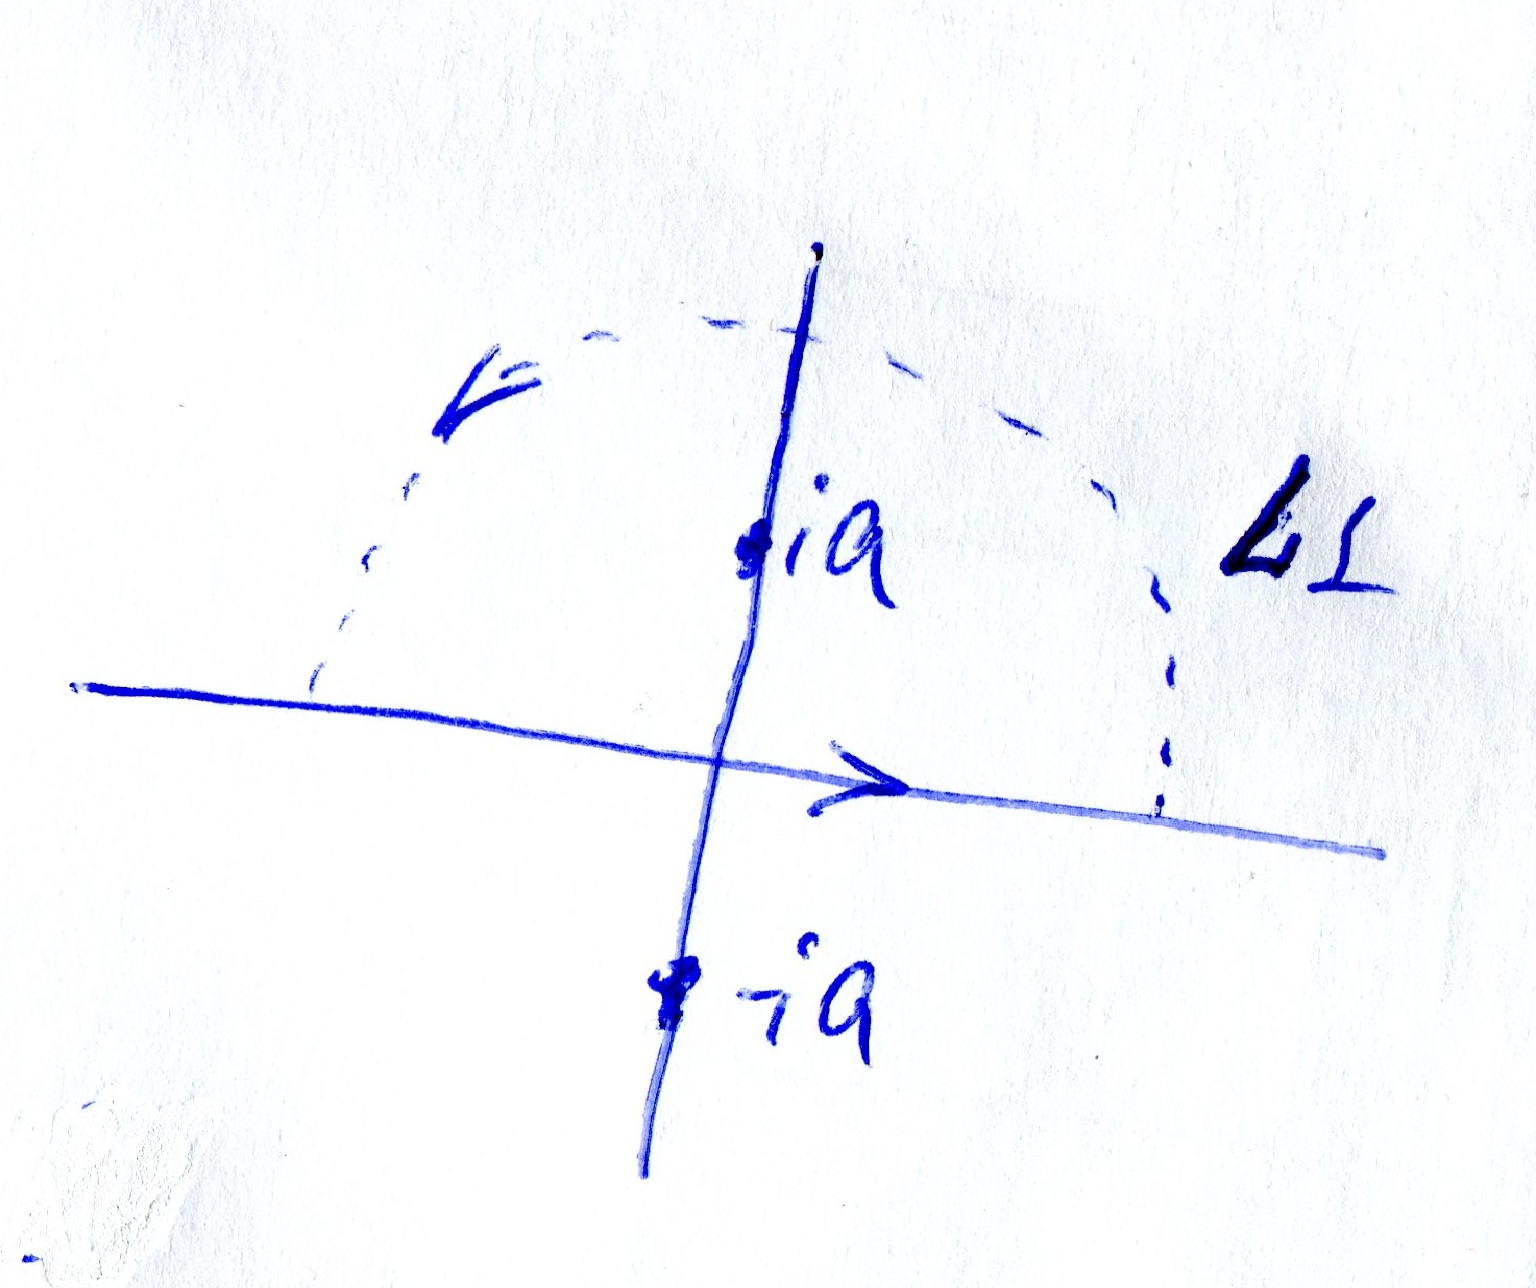
\includegraphics[width=\linewidth]{fig/fig83}
% \caption{}
% \vspace{-17pt}
% \end{wrapfigure}

$$res f(z) = \frac{\varphi(z_0)}{\psi^{'}(z_0)},$$
где $f(z)=R(z)\exp{i \lambda z}$, $z_0$-особая точка, $\varphi(z)=\frac{\exp{i \lambda z}}{z+ia}, \psi(z)=z-ia, \psi^{'}(z)=1$.
$$res f(ia) = \frac{e^{i \lambda i a}}{2ia}$$
$$\int_{-\infty}^{+\infty} \frac{1}{x^2+a^2} e^{\frac{-ipx}{\hbar}}dx=\frac{2\pi e^{\frac{ap}{\hbar}}}{2ia}=\frac{\pi}{a} e^{\frac{ap}{\hbar}}, p<0$$

1) $Im z<0, \lambda <0, p>0$.
$$\int_{-\infty}^{+\infty} \frac{1}{x^2+a^2} e^{\frac{-ipx}{\hbar}}dx=-2\pi i \sum_{k=1}^n res [R(z)\exp{i \lambda z}],$$
Внутри контура $L_2$ одна особая точка $z_0=-ia$

% \begin{wrapfigure}{l}{0.3\linewidth}
% 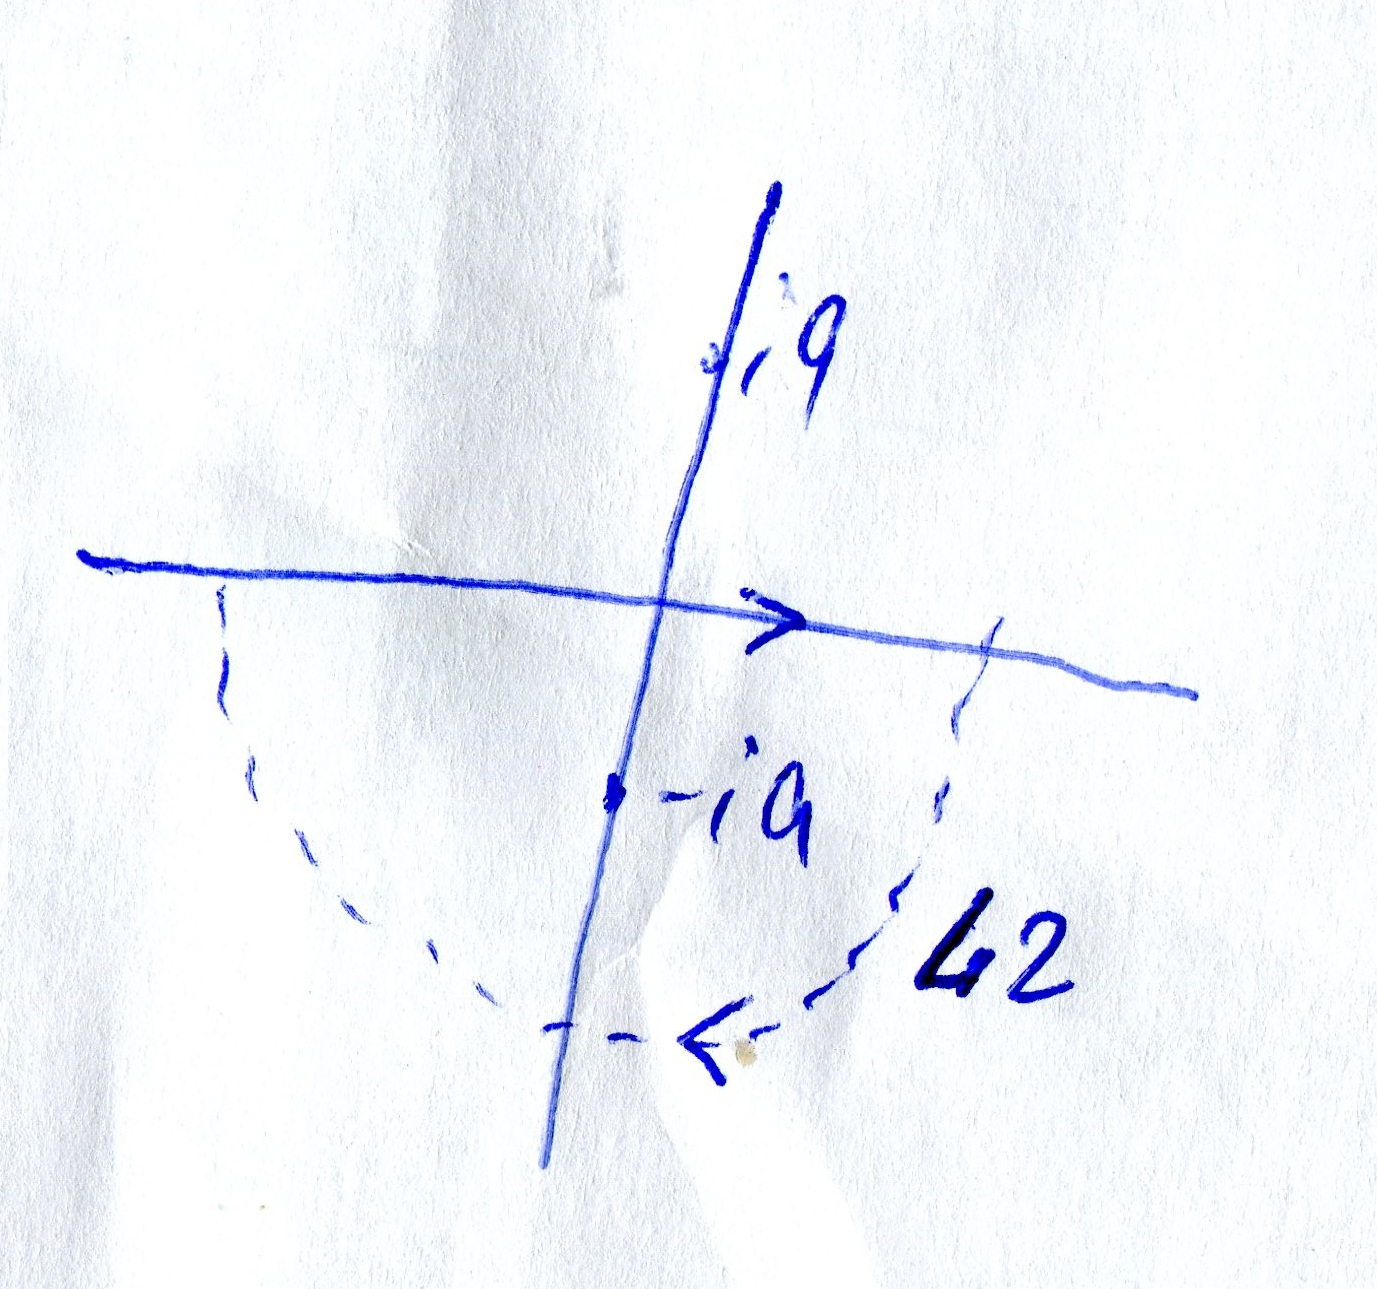
\includegraphics[width=\linewidth]{fig/fig831}
% \caption{}
% \vspace{-17pt}
% \end{wrapfigure}

$res f(z) = \frac{\varphi(z_0)}{\psi^{'}(z_0)}, \varphi(z)=\frac{\exp{i \lambda z}}{z-ia}, \psi(z)=z+ia, \psi^{'}(z)=1$.
$$res f(-ia) = \frac{e^{\lambda a}}{-2ia}$$
$$\int_{-\infty}^{+\infty} \frac{1}{x^2+a^2} e^{\frac{-ipx}{\hbar}}dx=\frac{-2\pi i e^{a\lambda}}{-2ia}=\frac{\pi}{a} e^{a\lambda}=\frac{\pi}{a} e^{\frac{-ap}{\hbar}}, p>0$$
$$\int_{-\infty}^{+\infty} \frac{1}{x^2+a^2} e^{\frac{-ipx}{\hbar}}dx=\frac{\pi}{a} e^{\frac{-a|p|}{\hbar}}$$
$$\Psi(p)=\frac{\pi}{a\sqrt{2\pi \hbar}}e^{\frac{-a|p|}{\hbar}}$$

Эта функция еще не нормирована. При нормировке амплитуда не важна.
 $$\Psi_0(p)=С e^{\frac{-a|p|}{\hbar}}$$
 $$\int_{-\infty}^{+\infty} |\Psi_0|^2 dp=C^2 \int_{-\infty}^{+\infty}e^{\frac{-a|p|}{\hbar}} dp= 2C^2 \int_{0}^{+\infty}e^{\frac{-ap}{\hbar}}dp=\frac{C^2\hbar}{a}$$
 Нормировка $\frac{C^2\hbar}{a}=1 \Longrightarrow C=\sqrt{\frac{a}{\hbar}}$ 
 $$\Psi_0(p)=\sqrt{\frac{a}{\hbar}} e^{\frac{-a|p|}{\hbar}}$$
 Найдем $\Delta p$ на уровне $e^{-1}$.
 $$-\frac{a|p^*|}{\hbar}=-1 \Longrightarrow p^*=\pm \frac{\hbar}{a} \Longrightarrow \Delta p=\frac{2\hbar}{a}$$
$\Delta x$ находится на уровне половины от максимума.
$$\Psi(x^*)=\frac{1}{2a^2}$$
$$\frac{1}{2a^2}=\frac{1}{x^{*2}+a^2} \Longrightarrow x^*=\pm a \Longrightarrow \Delta x=2a$$
$$\Delta x \cdot \Delta p= 4\hbar$$
 Соотношение неопределенностей позволяет проверить правильность решения. Произведение должно быть равно $\hbar$ с точностью до числового множителя.

